\section{Closed-loop Control over Wireless Networks}
The current generation of embedded wireless systems has largely focused on open-loop sensing and monitoring applications. To address actuation in closed-loop wireless control systems there is a strong need to re-think the communication architectures and protocols for reliability, coordination and control \cite{wireless-ind}.  Wireless networked control systems, or Networked Cyber-Physical Systems (Networked-CPS),  fundamentally differ from standard distributed systems in that the dynamics of the \emph{network} (variable channel capacity, probabilistic connectivity, topological changes, node and link failures) can change the operating points and physical dynamics of the \emph{closed-loop system}~\cite{ncs_stability, ncs_survey}. The most important objective of control in Networked-CPS is to provide stability of the closed-loop system. It is therefore necessary for the network (along with its interfaces to sensors and actuators) to be able to provide some form of guarantee of the control system's stability in the face of the non-idealities of the wireless links and the communication constraints of the wireless swarm network. A secondary goal in Networked-CPS is to allow for composition of additional controllers and plants within the same network without requiring reconfiguration of the entire network operation.

The most common approach to incorporating Networked-CPS into the feedback loop is to use it primarily as a communication medium: the nodes in the network simply route information to and from one or more \emph{dedicated controllers}, which are usually specialized CPUs capable of performing computationally expensive procedures (see \figref{wncs}). The use of dedicated controllers imposes a routing requirement along one or more fixed paths through the network, which must meet the stability constraints, encapsulated by end-to-end delay requirements~\cite{chenyang, evm_rtas10}. 
However, this assignment of routes is a static setup, which commonly requires global reorganization for changes in the underlying topology, node population and wireless link capacities. 

Routing couples the communication, computation and control problems \cite{alur_tac11,sched_TTA_HART,sched_TTA_scal}. Therefore, when a new route is required due to topological changes, the computation and control configurations must also be recalculated. Merely inserting a WNCS into the standard network architecture ``sensor $\rightarrow$ channel $\rightarrow$ controller/estimator $\rightarrow$ channel $\rightarrow$ actuator'' requires the addition of significant software support~\cite{evm_rtas10, etherware},  as the overhead of completely recomputing the computation and control configurations, due to topological changes or packet drops, is too expensive and does not scale.

 %%%%%%%%%%%%%%%%%%%%%%%%%%%%%%%%%%%%%%%%%%%%%%%%%%%%%%
\begin{figure*}[!t]
	\begin{center}
	`	\vspace{-5pt}
	\subfigure {%[\small (a) A wireless sensor, actuator and controller network. (b) Algorithm assignment to a set of controllers, each mapped to the respective nodes. (c) Three Virtual Components, each composed of several network elements.] {
	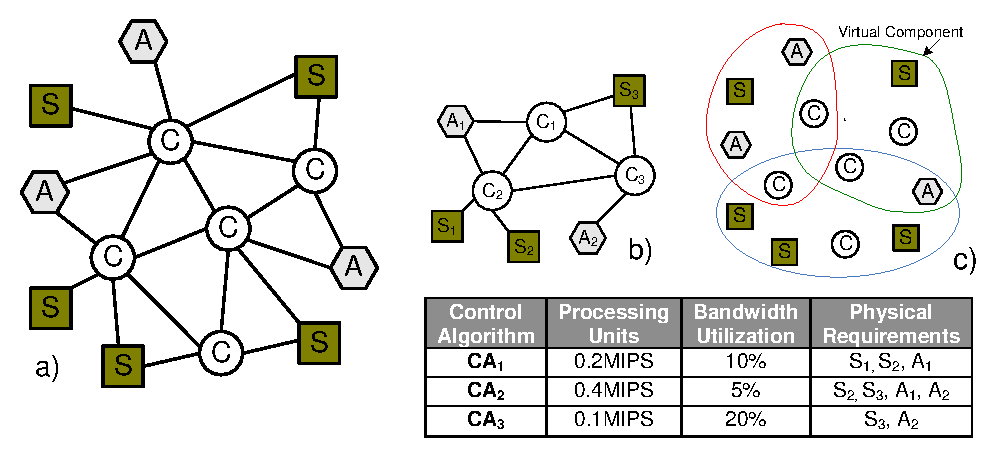
\includegraphics[width=0.55\textwidth]{figs/component_new.eps} 
  \vspace{-5pt}
	%\caption{\small (a) A wireless sensor, actuator and controller network. (b) Algorithm assignment to a set of controllers, each mapped to the respective nodes. (c) Three Virtual Components, each composed of several network elements.}
	\label{fig:component}
	}
	\hspace{.1in}
	\subfigure {%[(d) \small Decoupled virtual tasks and physical nodes with runtime task mapping.] {	
			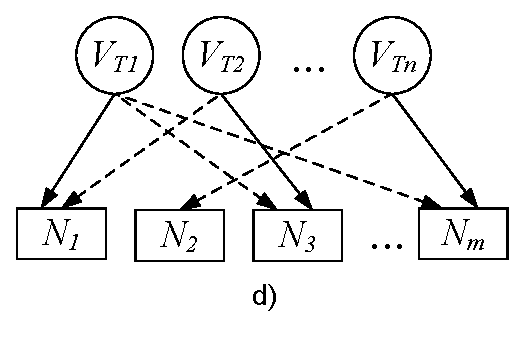
\includegraphics[width=0.3\textwidth]{figs/taskmap.eps}
			\label{fig:taskmap}
		}
	\end{center}	
\vspace{-15pt}
\caption{(a) A wireless sensor, actuator and controller network. (b) Algorithm assignment to a set of controllers, each mapped to the respective nodes. (c) Three Virtual Components, each composed of several network elements. (d) Decoupled virtual tasks and physical nodes with runtime task mapping.}
\label{fig:overview}
\vspace{-5pt}
\end{figure*}
%%%%%%%%%%%%%%%%%%%%%%%%%%%%%%%%%%%%%%%%%%%%%%%%%%%%%%

While providing a review of classical and recent approaches for control over wireless networks, we present two complementary approaches on maintaining stability in the presence of environment and network disturbances. The first approach adopts a ``computer systems" perspective on the design of robust architectures for embedded wireless control and actuation. We call this scheme Embedded Virtual Machines (see \figref{overview}) which provides software mechanisms to decouple controller functionality from the physical node - thus providing resilience to node, link and topology changes. The second approach adopts a ``control theoretic" perspective on distributed control within the network (see \figref{wcn}). This provides control mechanisms to remove controller functionality from a dedicated node to all nodes in the network - thus eliminating the need for routing and guaranteeing stability and optimal control in the presence of link, node and topology changes. 

\subsection{\textbf{Embedded Virtual Machines}}
Current approaches for robust networked control%algorithms
~\cite{ncs_survey} require the underlying network to satisfy a minimal set of requirements (e.g. guaranteed packet deliver rate, upper bound on network induced delay) and reduce the network model to that of a single channel with random delays. In addition, they do not address the spatial aspects of the network, i.e., how changes in the network topology affect the closed-loop system performance.

As the links, nodes and topology of wireless systems are inherently unreliable, such time-critical and safety-critical applications require programming abstractions where the tasks are assigned to the sensors, actuators and controllers as a \emph{single component}, rather than statically mapping a set of tasks to a specific physical node at design time (as shown in \figref{overview}). Such wireless controller grids are composed of many nodes that share a common sense of the control application but without regard to physical node boundaries. Our approach, is to \emph{decouple} the functionality (i.e., tasks) from the inherently unreliable physical substrate (i.e., nodes) and allow tasks to migrate/adapt (\figref{overview}(d)) to changes in the topology. 

To this end, we introduced the Embedded Virtual Machine (EVM), a powerful and flexible programming abstraction where a Virtual Component (VC) and its properties are maintained across node boundaries~\cite{evm_rtas10,evm_tecs11}, as shown in Fig. 2(c). EVMs differ from classical system virtual machines. In the enterprise or on PCs, one (powerful) physical machine may be partitioned to host multiple virtual machines for higher resource utilization. On the other hand, in the embedded domain, an EVM is composed across multiple physical nodes with the goal to maintain correct and high-fidelity operation even under changes in the physical composition of the network. The goal of the EVM is to maintain a set of \emph{functional invariants}, such as a control law and \emph{para-functional invariants} such as timeliness constraints, fault tolerance and safety standards across a set of controllers given the spatio-temporal changes in the physical network. Thus, the EVM introduces new degrees of freedom, task migration and routing which facilitates, at runtime, the network configuration (operating point, conditions) to meet the requirements of the networked control algorithms. However, the EVM does not provide explicit guarantees but only finds the optimal operation configuration in terms of routing and task assignment.

\subsection{\textbf{Distributed Control over Wireless Networks}}
Let us consider the problem of stabilizing a plant with a multi-hop network of resource constrained wireless nodes. 
In ~\cite{wcn_tac11}, we introduced the concept of a {\it Wireless Control Network} (WCN), which is a paradigm change for distributed control over a wireless network. In a WCN the entire network {\it itself} acts as a controller, as the computation is spread over the whole network, instead of assigning a particular node with the execution of the control procedure.  We have devised a numerical design procedure that produces the coefficients of the linear combinations for each node and actuator to apply in order to stabilize the plant.  The radio connectivity between nodes in the network induces topological constraints to the control algorithm, and this topology determines whether it is even possible to stabilize the system with the use of linear iterative strategies.  In addition, a method to synthesize an optimal WCN, with respect to the standard cost functions, has been developed~\cite{JIISc_distrCPS}. 

Given the fundamental unreliability of wireless communication, the WCN method handles topological constraints while maintaining mean square stability for packet drop rates \textbf{\emph{up to 20\%}} for a specific network topology and plant. This bridges the gap between the basic WCN and the theoretical upper bound of robustness to packet drops~\cite{Hadjicostis02}. We also show a method to synthesize a WCN robust to a certain level of node failures, and then extend the synthesis procedures to allow for the use of the WCN for control of continuous-time plants. 

While in the past efforts, we consider scenarios where the network topology is already set, in recent efforts~\cite{wcn_jsac12, wcn_cdc11} we have investigated a dual problem, ``how to synthesize the network so that a stable WCN configuration exists?" The topological conditions from~\cite{wcn_jsac12}, along with the results from~\cite{wcn_tac11} provide the essential building blocks for an integrated decentralized wireless control network design framework. Early experiments in an industrial process control case study of a distillation column in a process-in-the-loop test-bed demonstrate optimal control of continuous-time physical processes which maintain system stability under the presence of node and link failures. 

\subsubsection{Advantages of the WCN}
The WCN introduces very low communication and computation overhead. The linear iterative runtime procedure is computationally very inexpensive as each node only computes a linear combination of its value and values of its neighbors. This makes it suitable for resource constrained, low-power wireless nodes (e.g., Tmote).
Furthermore, the communication overhead is also very small, as each node needs to transmit only its own state once per frame.  In the case when a node maintains a scalar state it transmits only \emph{2 bytes} in each message, making it suitable to combine this scheme with periodic message transmissions in existing wireless systems. 

The WCN utilizes a simple transmission schedule where each node is active only once during a TDMA cycle and the control-loop does not impose end-to-end delay requirements. This allows the network operator to decouple the computation schedule from the communication schedule, which significantly simplifies closed-loop system design and enables compositional design and analysis. 